% This file describes the general structure of some of our tb_dynamics models.
% Note that it is possible to construct models in many different ways using the tb_dynamics code.
% Therefore, this description should be used with caution, because it only describes one possible model configuration.

\section{Model Structure}

\subsection{General features}

We use a deterministic compartmental model including six types of compartments that represent 
different states of infection and disease. The model uses the same conceptual approach and similar 
assumptions to previously published models \cite{trauer-2017, ragonnet-2019, ragonnet-2021, ragonnet-2022}. 
Here we describe the model structure before applying any stratification. 
\newline
A susceptible compartment (S) is used to represent individuals who have 
never been infected with Mycobacterium tuberculosis (M.tb). Latent TB infection (LTBI) is modelled 
using two successive compartments: early latent (E) and late latent (L) to capture the declining risk of 
disease progression over time from infection \cite{ragonnet-2017}. The active disease compartment (I) represents 
individuals who have progressed to the active stage of TB disease. Diseased individuals who recover 
through self-cure progress directly to the recovered compartment (R). All diseased individuals who 
are detected are assumed to be started on treatment (compartment T). Treatment may result in cure 
(progression to R), relapse (return to I) or death.
\newline
Non-TB-related mortality is modelled by applying death rates to all model compartments. In addition, 
disease-specific mortality is implemented by applying increased mortality rates to the active disease 
compartments (I and T).
\newline
Reinfection occurs in the model in two different ways. First, latently infected individuals may be 
reinfected, with this process modelled using a flow from the late latent (L) to the early latent 
compartment (E). Second, individuals who have recovered from TB disease may be reinfected and 
return to the early latent compartment. The structure of our model allows for differential risk of 
infection for the currently and previously infected individuals, compared to the infection-naive 
individuals.
\begin{figure}[!htbp]
    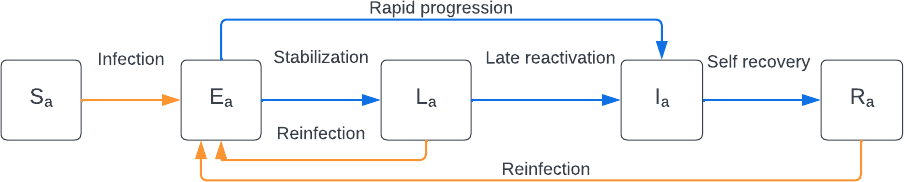
\includegraphics[width=\textwidth,height=\textheight,keepaspectratio]{model.png}
    \caption{TIllustration of the model structure. 
    Boxes represent the different compartments types: susceptible (S), early latent (E), late latent (L), infectious (I), on treatment (T) and recovered (R). The subscripts indicate whether compartments are stratified by age (a), geography (g) and form of tuberculosis (f). Blue and orange arrows represent progression flows and transmission flows, respectively. 
    The flows associated with the modelled interventions are shown in purple. ACF, active case finding.}
    \label{fig:model}
\end{figure}

